%\documentclass[border=10pt]{standalone}
%\usepackage{tikz}
\tikzset{
	treenode/.style = {shape=rectangle, rounded corners,
		draw, align=center,
		top color=white, bottom color=blue!20},
	root/.style     = {treenode, font=\ttfamily\normalsize},
	env/.style      = {treenode, font=\ttfamily\normalsize},
	dummy/.style    = {circle,draw},
	level 1/.style={sibling distance=6cm, level distance = 1em},
	level 2/.style={sibling distance=2.5cm,level distance = 5em}, 
	level 3/.style={sibling distance=2cm},
	blueRed/.style={env, top color=blue, bottom color=red} 
}
%\begin{document}
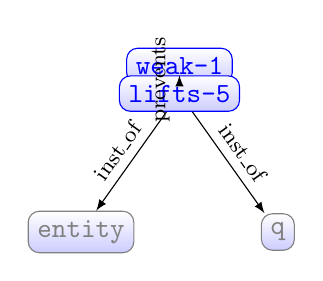
\begin{tikzpicture}
[
grow                    = down,
sibling distance        = 50em,
level distance          = 5em,
edge from parent/.style = {draw, -latex},
every node/.style       = {font=\footnotesize},
sloped
]
\node  [env, blue] {weak-1}
child { node [env, blue] {lifts-5}
	child {node [env, gray] {entity}
		edge from parent node [above] {inst\_of}}
	child {node [env, gray] {q}
		edge from parent node [above] {inst\_of}} 	
	edge from parent node [above] {prevents}};


\end{tikzpicture}
%\end{document}